\documentclass[10pt]{article}
\usepackage[paperwidth=13.333in,paperheight=7.5in,margin=0in]{geometry}
\usepackage{fontspec}
\usepackage{xcolor}
\usepackage{graphicx}
\usepackage{amsfonts}
\usepackage{array}
\usepackage{tabularx}

\setsansfont[
  Path=fonts/,
  UprightFont=FreeSans.ttf,
  BoldFont=FreeSansBold.ttf,
  ItalicFont=FreeSansOblique.ttf
]{FreeSans}
\renewcommand{\familydefault}{\sfdefault}

\definecolor{DeepPurple}{HTML}{2B1E3E}
\definecolor{CosmicBlue}{HTML}{4A4E8F}
\definecolor{Lavender}{HTML}{A490C2}
\definecolor{Silver}{HTML}{E6E6FA}
\definecolor{Obsidian}{HTML}{171A24}
\definecolor{MineralCyan}{HTML}{4FC3C8}
\definecolor{EmberGold}{HTML}{D6A34A}
\definecolor{Moss}{HTML}{79A879}
\definecolor{Warning}{HTML}{D9A441}
\definecolor{Paper}{HTML}{F7F5FB}
\pagecolor{DeepPurple}
\color{Silver}

\setlength{\parindent}{0pt}
\setlength{\parskip}{4pt}
\setlength{\fboxsep}{0pt}
\pagestyle{empty}
% Archivo generado por scripts/build_presentation.py. No editar a mano.
\newif\iftrainingcomplete
\trainingcompletefalse
\newif\ifgalleryready
\galleryreadyfalse
\newcommand{\TargetEpochs}{60}
\newcommand{\BaselineEpoch}{1}
\newcommand{\BaselineLossD}{0.1156}
\newcommand{\BaselineLossG}{8.5477}
\newcommand{\BaselineDiversity}{0.0551}
\newcommand{\HingeEpoch}{1}
\newcommand{\HingeLossD}{0.2482}
\newcommand{\HingeLossG}{15.2575}
\newcommand{\HingeDiversity}{0.0860}
\newcommand{\SpectralEpoch}{1}
\newcommand{\SpectralLossD}{0.0760}
\newcommand{\SpectralLossG}{6.8625}
\newcommand{\SpectralDiversity}{0.0618}
\newcommand{\FinalExperiment}{pendiente}
\newcommand{\SelectionRate}{10/200 = 5\% planificado}
\newcommand{\MeanNeighborSimilarity}{pendiente}
\newcommand{\HardestCharacter}{pendiente}
\newcommand{\HardestSimilarity}{pendiente}
\newcommand{\RegenerationDelta}{pendiente}


\newcommand{\slide}[2]{%
  \clearpage
  \thispagestyle{empty}
  \noindent\colorbox{Obsidian}{%
    \parbox[c][0.86in][c]{\paperwidth}{%
      \hspace*{0.55in}{\fontsize{25}{29}\selectfont\bfseries\color{Silver}#1}%
    }%
  }
  \vspace{0.22in}
  \hspace*{0.55in}\begin{minipage}[t][5.85in][t]{12.23in}
    #2
  \end{minipage}
  \vfill
  \hspace*{0.55in}{\scriptsize\color{Lavender}ERYNDOR · GUARDIANES DEL VELO}
  \hfill{\scriptsize\color{Lavender}\thepage/12}\hspace*{0.55in}
  \vspace{0.16in}
}

\newcommand{\eyebrow}[1]{{\fontsize{10}{12}\selectfont\bfseries\color{MineralCyan}\MakeUppercase{#1}}}
\newcommand{\bigstat}[2]{%
  \colorbox{CosmicBlue}{\parbox[c][0.88in][c]{2.55in}{\centering
    {\scriptsize\color{Silver}#1}\\[-1pt]
    {\fontsize{21}{24}\selectfont\bfseries\color{white}#2}}}%
}
\newcommand{\statuspending}[1]{%
  \colorbox{Obsidian}{\parbox[c][2.7in][c]{11.4in}{\centering
    {\fontsize{28}{32}\selectfont\bfseries\color{EmberGold}EVIDENCIA PENDIENTE}\\[8pt]
    {\large\color{Silver}#1}\\[12pt]
    {\small\color{Lavender}El pipeline bloquea resultados incompletos y no escribe una galería falsa.}}}%
}
\newcommand{\pill}[1]{\colorbox{CosmicBlue}{\strut\hspace{7pt}\color{white}\bfseries #1\hspace{7pt}}}
\newcommand{\metricrow}[4]{#1 & #2 & #3 & #4\\}

\begin{document}

% 1
\clearpage
\thispagestyle{empty}
\noindent\colorbox{Obsidian}{\parbox[c][\paperheight][c]{\paperwidth}{
\hspace*{0.72in}\begin{minipage}{11.7in}
  \eyebrow{Deep Learning 2026 · Proyecto 2}\par
  \vspace{0.22in}
  {\fontsize{42}{46}\selectfont\bfseries\color{white}Eryndor}\par
  {\fontsize{29}{34}\selectfont\bfseries\color{Lavender}Guardianes del Velo}\par
  \vspace{0.22in}
  {\Large\color{Silver}Diseño generativo de personajes para un RPG de aventura y magia}\par
  \vspace{0.55in}
  \bigstat{DATOS}{4,096}\hspace{0.16in}
  \bigstat{RESOLUCIÓN}{64 × 64}\hspace{0.16in}
  \bigstat{EXPERIMENTOS}{3}\hspace{0.16in}
  \ifgalleryready\bigstat{GALERÍA}{10 / 200}\else\bigstat{META GALERÍA}{10 / 200}\fi\par
  \vspace{0.62in}
  {\large\bfseries\color{MineralCyan}Pablo Daniel Barillas Moreno · Wilson Alejandro Calderón}\par
  {\normalsize\color{Lavender}Universidad del Valle de Guatemala · Sección 30}\par
  \vspace{0.25in}
  {\small\color{Silver}Presentación regenerable desde métricas, checkpoint y vectores latentes.}
\end{minipage}}}

% 2
\slide{01 · Un universo fracturado por magia mineral}{
\begin{minipage}[t]{7.55in}
  \eyebrow{Dirección creativa}\par
  \vspace{0.1in}
  {\fontsize{21}{25}\selectfont\bfseries\color{white}Aventura melancólica, materiales gastados\\y esperanza contenida.}\par
  \vspace{0.22in}
  Eryndor quedó dividido por la \textbf{Ruptura Celeste}. Sus guardianes exploran ruinas, recuperan reliquias y contienen grietas arcanas. La GAN debe producir sprites que parezcan sobrevivientes del mismo mundo, no fantasía genérica.
  \vspace{0.25in}
  \begin{tabular}{@{}p{1.65in}p{5.45in}@{}}
    \color{MineralCyan}\bfseries Perspectiva & Cuerpo completo, ortográfica elevada, pose frontal consistente.\\[5pt]
    \color{MineralCyan}\bfseries Materiales & Metal, cuero, tela, madera y cristal mágico.\\[5pt]
    \color{MineralCyan}\bfseries Acentos & Cian mineral, oro brasa y amatista sobre fondo obsidiana.\\[5pt]
    \color{MineralCyan}\bfseries Roles & Guardián rúnico, arcanista, explorador, alquimista y oráculo.\\
  \end{tabular}
\end{minipage}\hfill
\begin{minipage}[t]{4.25in}
  \colorbox{CosmicBlue}{\parbox[c][4.45in][c]{4.25in}{\centering
    {\fontsize{17}{21}\selectfont\bfseries\color{white}Criterio de éxito}\\[14pt]
    {\large\color{Silver}10 personajes distintos}\\[7pt]
    {\large\color{Silver}e inexistentes}\\[18pt]
    {\color{Lavender}+ evolución con ruido fijo}\\[5pt]
    {\color{Lavender}+ curvas interpretadas}\\[5pt]
    {\color{Lavender}+ vecinos cercanos}\\[5pt]
    {\color{Lavender}+ regeneración exacta}\\[18pt]
    \pill{Sin generadores externos}
  }}
\end{minipage}
}

% 3
\slide{02 · Datos abiertos, consistentes y auditados}{
\begin{minipage}[t]{6.55in}
  \vspace{0pt}
  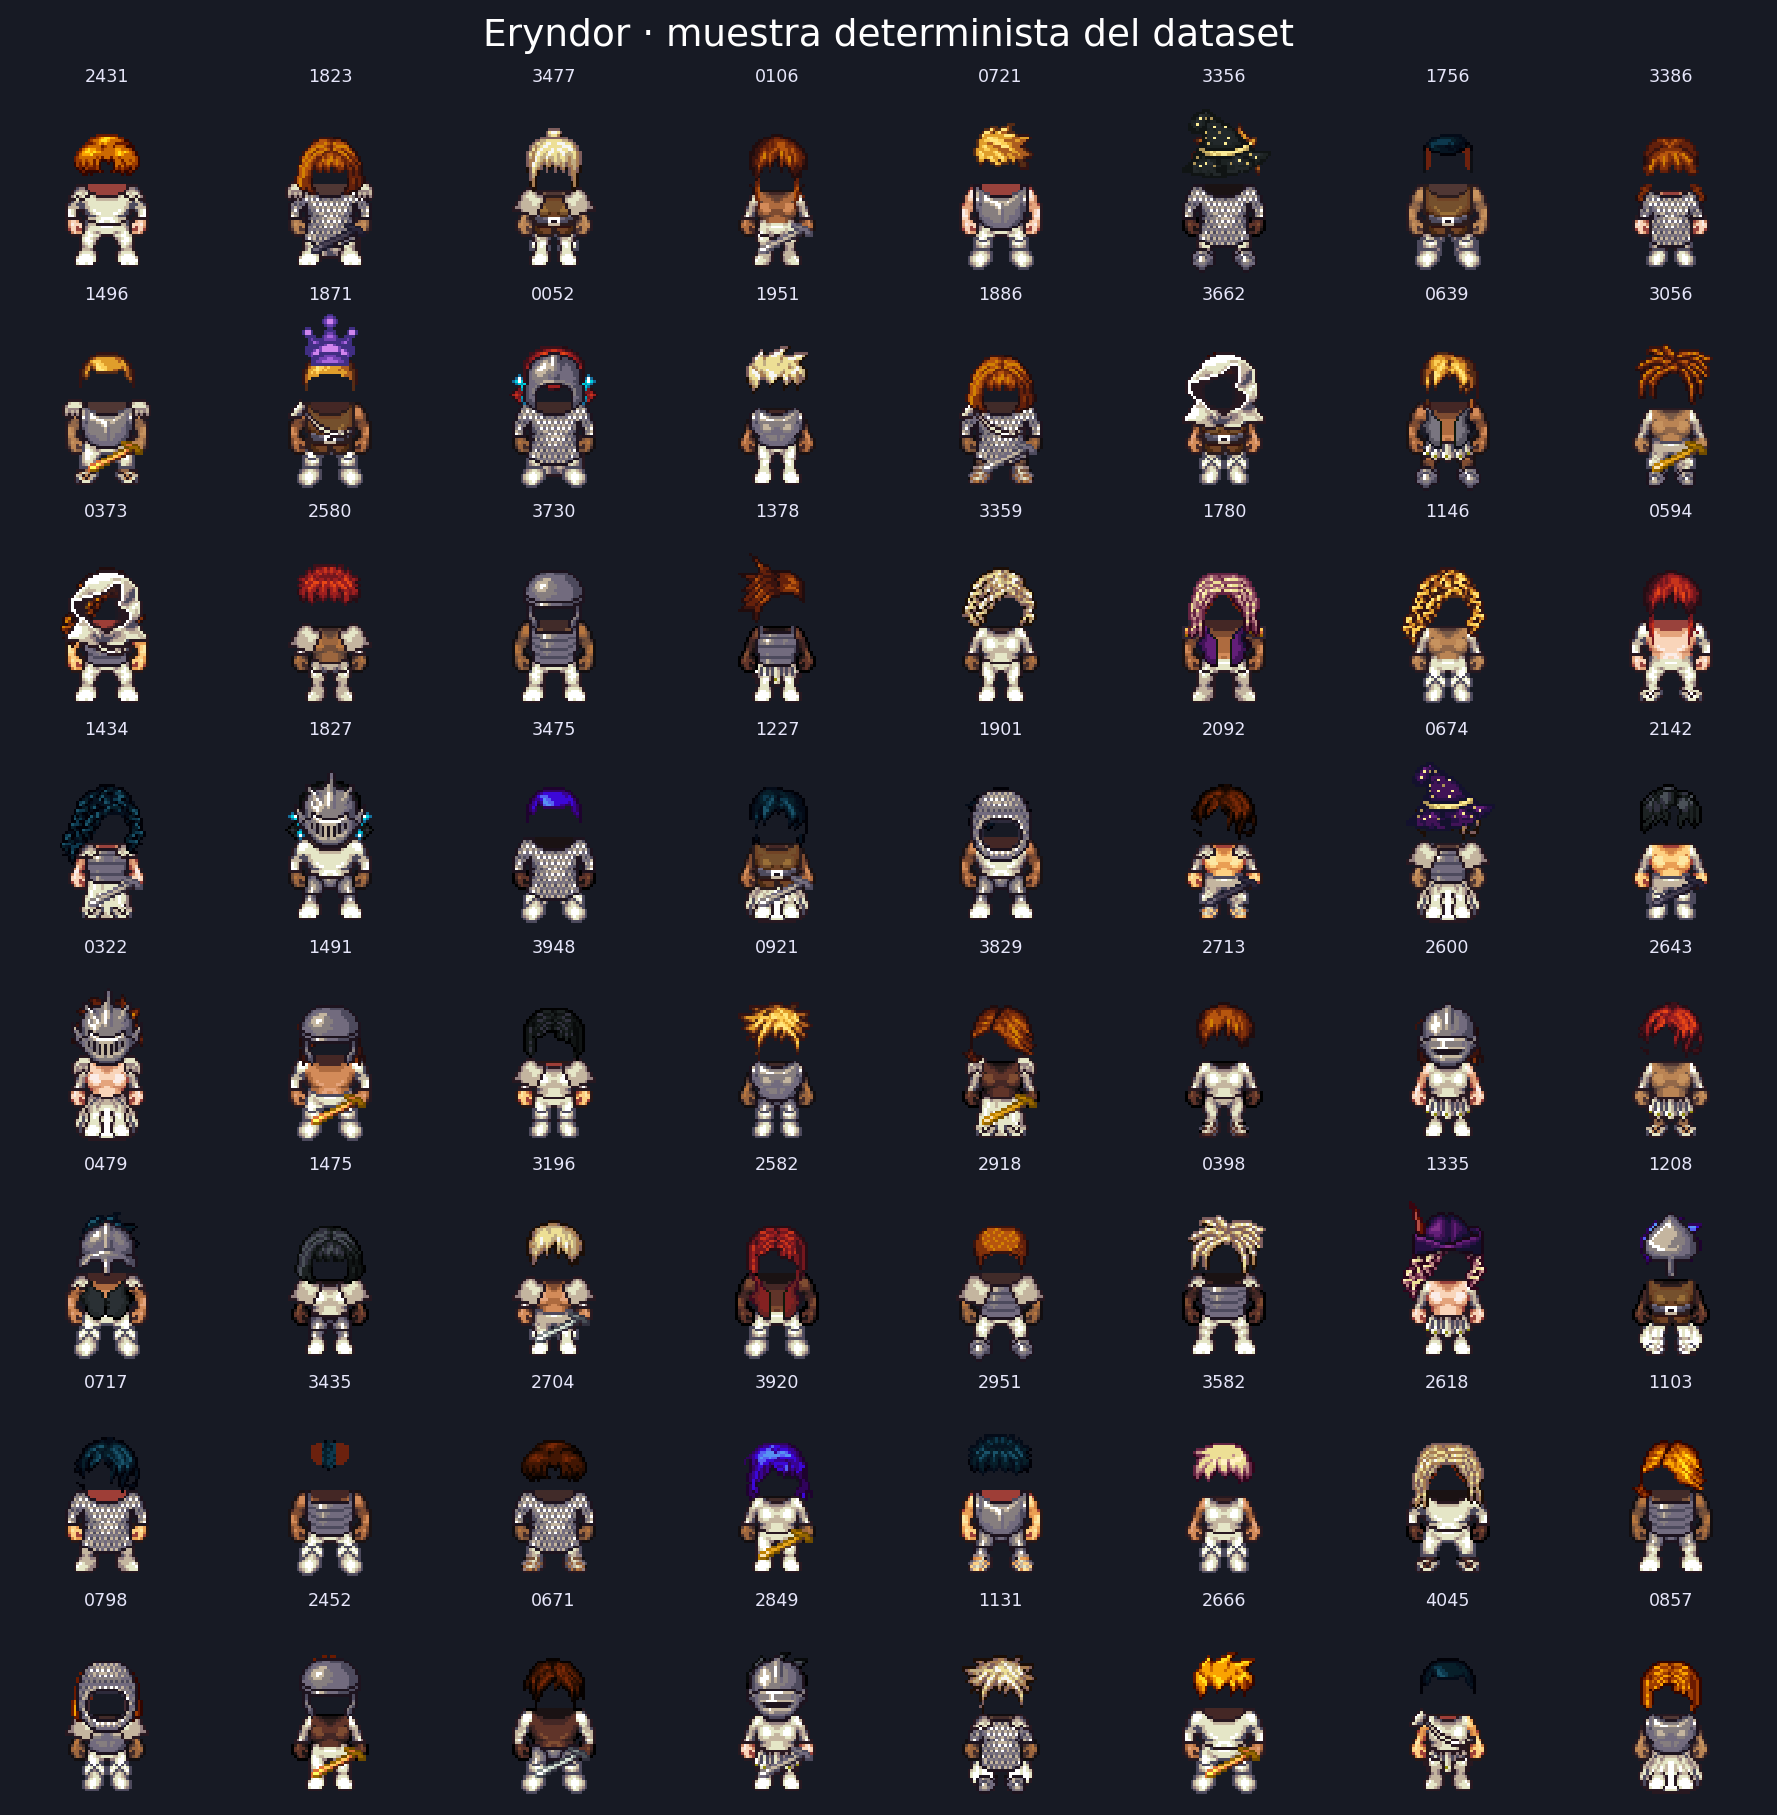
\includegraphics[width=6.45in,height=4.55in,keepaspectratio]{../artifacts/dataset/dataset_contact_sheet.png}
  \par{\scriptsize\color{Lavender}Muestra determinista del conjunto LPC preparado por el equipo.}
\end{minipage}\hfill
\begin{minipage}[t]{5.25in}
  \eyebrow{Liberated Pixel Cup}\par
  \vspace{0.08in}
  \begin{tabular}{@{}p{2.65in}r@{}}
    Imágenes RGB & \textbf{4,096}\\[4pt]
    Resolución & \textbf{64 × 64}\\[4pt]
    Duplicados SHA-256 & \textbf{0}\\[4pt]
    Archivos faltantes & \textbf{0}\\[4pt]
    Estilos de cabello & \textbf{44}\\[4pt]
    Estilos de torso & \textbf{18}\\[4pt]
    Ocupación media & \textbf{23.18\%}\\[4pt]
    Capas acreditadas & \textbf{254/254}\\
  \end{tabular}\par
  \vspace{0.18in}
  \colorbox{Obsidian}{\parbox{4.95in}{\vspace{8pt}\hspace{9pt}\parbox{4.55in}{\small
    \textbf{Preparación:} composición por capas, cuadro frontal, fondo \texttt{\#171A24}, RGB, normalización a $[-1,1]$ y flip horizontal $p=0.5$.\\[5pt]
    \textbf{Licencias:} CC0, CC-BY, CC-BY-SA, OGA-BY y GPL con atribución por capa.
  }\vspace{8pt}}}\par
  \vspace{0.13in}
  {\scriptsize\color{Lavender}Fuente: Universal LPC Spritesheet Character Generator, commit 4963a697.}
\end{minipage}
}

% 4
\slide{03 · DCGAN: una base simple y explicable}{
\eyebrow{Arquitectura 64 × 64}\par
\vspace{0.12in}
\begin{minipage}[t]{5.72in}
  \colorbox{CosmicBlue}{\parbox[c][3.58in][c]{5.72in}{\hspace{0.25in}\parbox{5.18in}{
    {\Large\bfseries\color{white}Generador G}\par\vspace{0.15in}
    $z\in\mathbb{R}^{128}\rightarrow 512\rightarrow256\rightarrow128\rightarrow64\rightarrow3$\\[8pt]
    Cinco convoluciones transpuestas; BatchNorm + ReLU en bloques internos y \texttt{tanh} en RGB.\\[12pt]
    \textbf{Salida:} $[B,3,64,64]$ en $[-1,1]$\\[6pt]
    \textbf{Parámetros:} 3,806,080
  }}}
\end{minipage}\hfill
\begin{minipage}[t]{5.72in}
  \colorbox{Obsidian}{\parbox[c][3.58in][c]{5.72in}{\hspace{0.25in}\parbox{5.18in}{
    {\Large\bfseries\color{MineralCyan}Discriminador D}\par\vspace{0.15in}
    $3\rightarrow64\rightarrow128\rightarrow256\rightarrow512\rightarrow1$\\[8pt]
    Cinco convoluciones; LeakyReLU 0.2; BatchNorm desde el segundo bloque; salida en logits.\\[12pt]
    \textbf{Salida:} $[B]$, sin sigmoide interno\\[6pt]
    \textbf{Parámetros:} 2,765,568
  }}}
\end{minipage}\par
\vspace{0.28in}
\colorbox{DeepPurple}{\parbox{11.75in}{\centering\large
  Adam · $lr=2\times10^{-4}$ · $\beta=(0.5,0.999)$ · batch 64 · semilla 42 · 60 épocas
}}
}

% 5
\slide{04 · Experimentos: una variable a la vez}{
\eyebrow{Protocolo pre-registrado}\par
\vspace{0.14in}
\begin{tabularx}{11.95in}{>{\bfseries\color{MineralCyan}}p{0.45in} p{1.75in} p{2.1in} X}
  ID & Pérdida & Estabilización & Hipótesis previa\\[4pt]
  \hline\\[-8pt]
  A & BCE no saturante & Baseline & Producirá siluetas reconocibles por la consistencia del dataset.\\[7pt]
  B & Hinge loss & Igual a A & Mantendrá gradientes útiles y puede mejorar nitidez y diversidad.\\[7pt]
  C & BCE no saturante & Spectral norm en D & Limitará a D y reducirá periodos prolongados de dominio.\\
\end{tabularx}
\vspace{0.32in}
\colorbox{Obsidian}{\parbox[c][1.55in][c]{11.95in}{\hspace{0.28in}\parbox{11.35in}{
  \textbf{Control común:} mismos datos, arquitectura, semillas, optimizadores, 60 épocas y 16 vectores de ruido fijo.\\[8pt]
  \textbf{Criterio:} no elegir por una sola pérdida; combinar evolución visual, diversidad, vecinos, coherencia y ausencia de colapso.
}}}
\vspace{0.28in}
\pill{A → control}\hspace{0.2in}\pill{B → cambia pérdida}\hspace{0.2in}\pill{C → cambia estabilización}
}

% 6
\slide{05 · Evidencia 1: el mismo ruido a través del tiempo}{
\begin{minipage}[t]{8.5in}
  \vspace{0pt}
  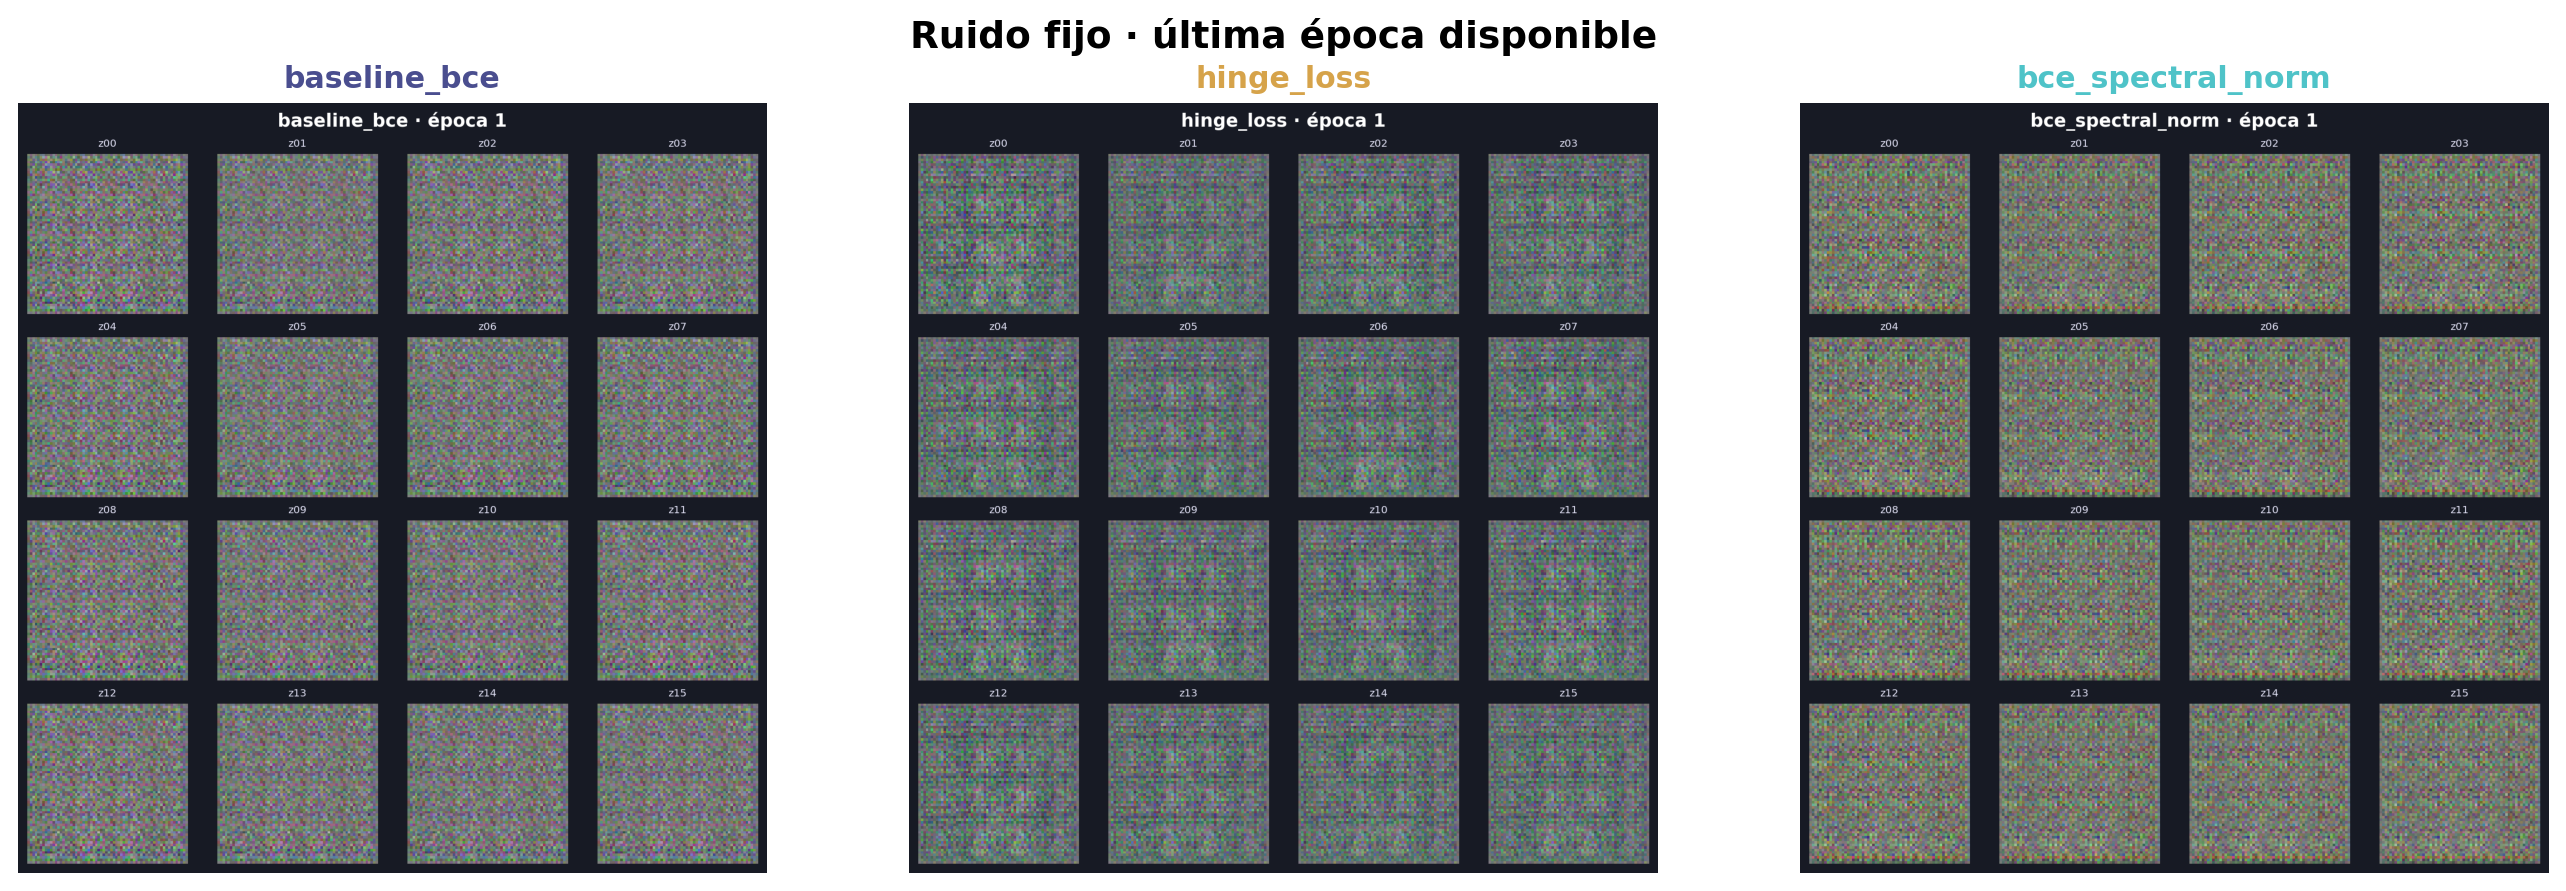
\includegraphics[width=8.35in,height=4.75in,keepaspectratio]{../artifacts/experiments/latest_fixed_noise_comparison.png}
\end{minipage}\hfill
\begin{minipage}[t]{3.25in}
  \eyebrow{Estado actual}\par
  \vspace{0.12in}
  {\fontsize{24}{28}\selectfont\bfseries\color{EmberGold}1 / 60}\par
  {\small épocas por experimento}\par
  \vspace{0.2in}
  Las tres rejillas siguen dominadas por textura de alta frecuencia. No hay personajes reconocibles todavía.
  \vspace{0.2in}
  \colorbox{Obsidian}{\parbox{3.0in}{\vspace{8pt}\hspace{8pt}\parbox{2.7in}{\small
    Se conservarán hitos en 0, 5, 10, 20, 40 y 60 para detectar convergencia o colapso.
  }\vspace{8pt}}}\par
  \vspace{0.18in}
  {\small\color{MineralCyan}\bfseries Interpretación honesta:}\par
  Una época valida el pipeline, no la calidad final.
\end{minipage}
}

% 7
\slide{06 · Evidencia 2: dinámica adversarial observada}{
\begin{minipage}[t]{6.55in}
  \vspace{0pt}
  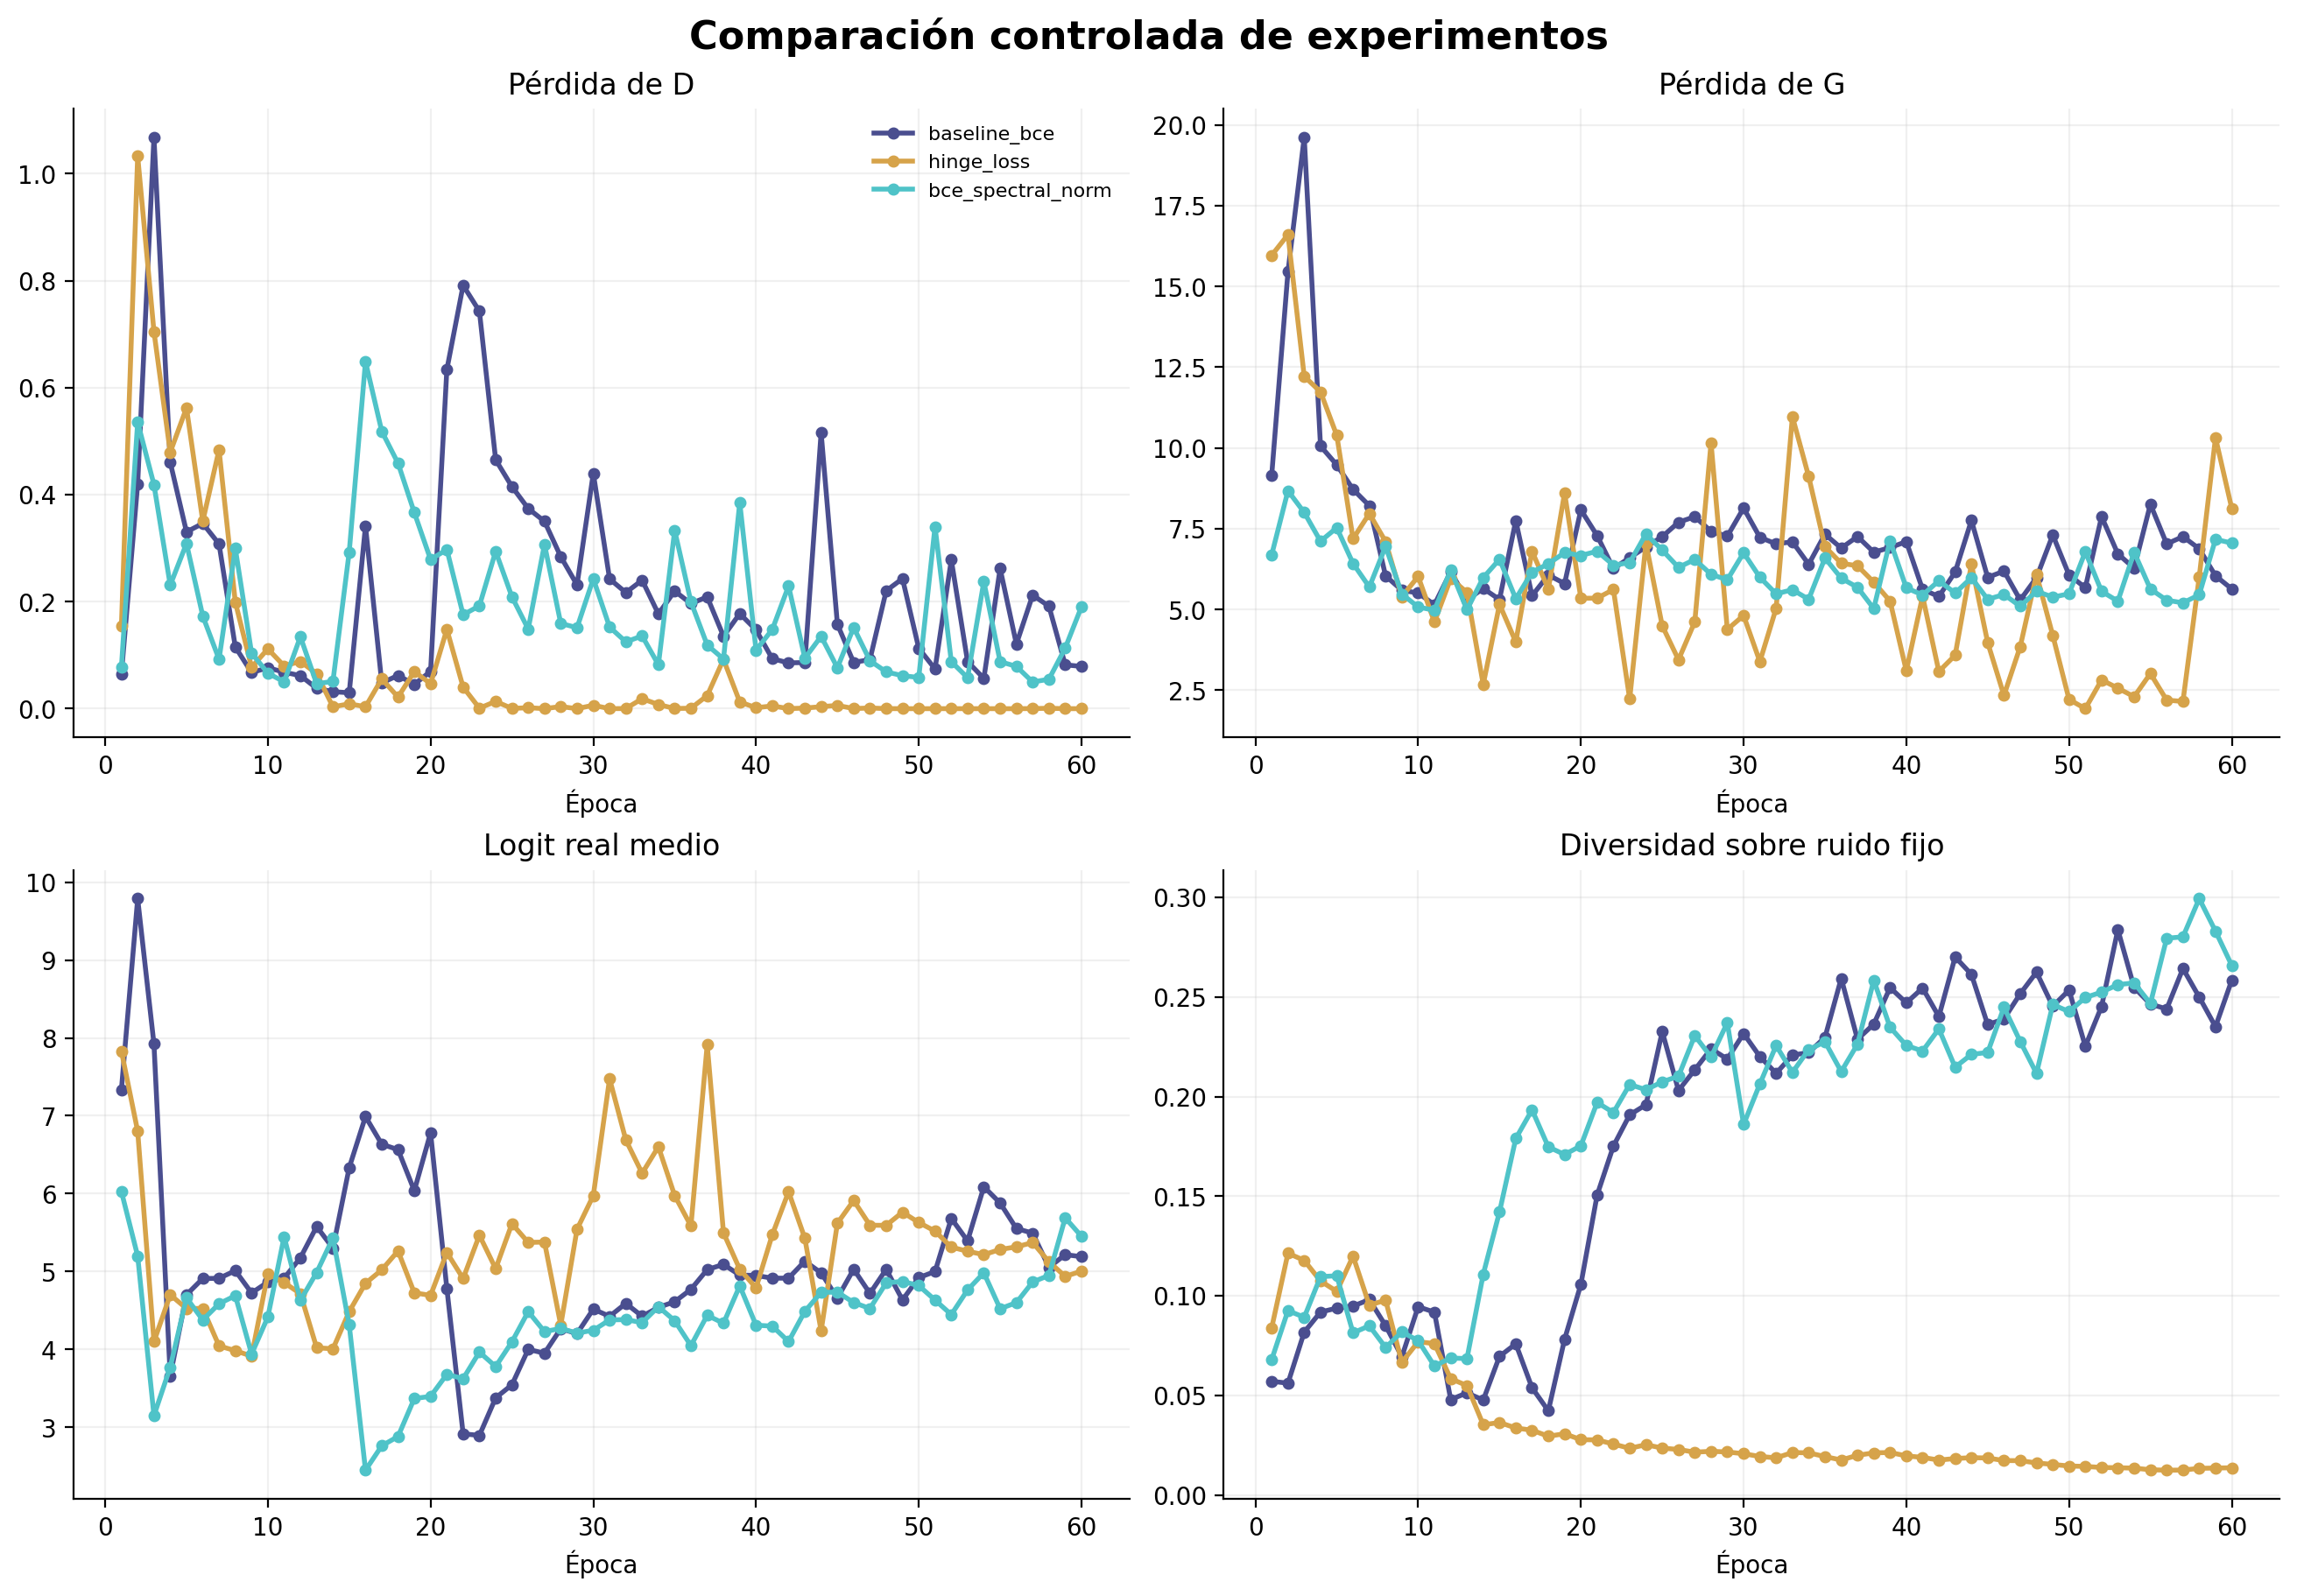
\includegraphics[width=6.45in,height=4.4in,keepaspectratio]{../artifacts/experiments/experiment_comparison.png}
\end{minipage}\hfill
\begin{minipage}[t]{5.25in}
  \eyebrow{Última época disponible}\par
  \vspace{0.1in}
  \small
  \begin{tabular}{@{}p{1.45in}r r r@{}}
    & $L_D$ & $L_G$ & diversidad\\[3pt]
    \metricrow{BCE}{\BaselineLossD}{\BaselineLossG}{\BaselineDiversity}
    \metricrow{Hinge}{\HingeLossD}{\HingeLossG}{\HingeDiversity}
    \metricrow{Spectral}{\SpectralLossD}{\SpectralLossG}{\SpectralDiversity}
  \end{tabular}\par
  \vspace{0.22in}
  \colorbox{Obsidian}{\parbox{4.95in}{\vspace{8pt}\hspace{9pt}\parbox{4.55in}{\small
    \textbf{Lectura:} D separó rápidamente reales y falsos. Hinge mostró la mayor distancia fija inicial, pero BCE y hinge tienen escalas distintas y 1 época no permite un ranking.
  }\vspace{8pt}}}\par
  \vspace{0.18in}
  \iftrainingcomplete
    {\color{Moss}\bfseries Entrenamiento completo; interpretar la trayectoria total.}
  \else
    {\color{EmberGold}\bfseries Resultado parcial: las comparaciones finales siguen bloqueadas.}
  \fi
\end{minipage}
}

% 8
\slide{07 · Estabilidad, fallos y decisiones}{
\begin{minipage}[t]{5.72in}
  \eyebrow{Señales observadas}\par
  \vspace{0.12in}
  \colorbox{Obsidian}{\parbox[c][3.75in][c]{5.72in}{\hspace{0.25in}\parbox{5.15in}{
    {\large\bfseries\color{EmberGold}Discriminador dominante al inicio}\par
    En el smoke test, $L_D$ cayó de 1.879 a 0.153 y $L_G$ subió de 4.970 a 7.522.\\[13pt]
    {\large\bfseries\color{EmberGold}Rejillas todavía ruidosas}\par
    Ninguna variante genera una silueta defendible en la época 1.\\[13pt]
    {\large\bfseries\color{EmberGold}Mode collapse}\par
    Aún no puede diagnosticarse; se monitorea con ruido fijo y distancia entre muestras.
  }}}
\end{minipage}\hfill
\begin{minipage}[t]{5.72in}
  \eyebrow{Controles implementados}\par
  \vspace{0.12in}
  \colorbox{CosmicBlue}{\parbox[c][3.75in][c]{5.72in}{\hspace{0.25in}\parbox{5.15in}{
    \textbf{1.} Spectral normalization solo en D.\\[10pt]
    \textbf{2.} Checkpoints reanudables con RNG, optimizadores y orden de datos.\\[10pt]
    \textbf{3.} Métricas por paso/época y ruido fijo común.\\[10pt]
    \textbf{4.} Galería bloqueada antes de época 60.\\[10pt]
    \textbf{5.} Selección 10/200, vecinos ResNet18 y regeneración exacta.
  }}}
\end{minipage}\par
\vspace{0.28in}
{\large\bfseries\color{MineralCyan}Un resultado que no mejora también es válido si el control y el análisis son honestos.}
}

% 9
\slide{08 · Galería final: diez guardianes de Eryndor}{
\ifgalleryready
  \begin{minipage}[t]{9.05in}
    \vspace{0pt}
    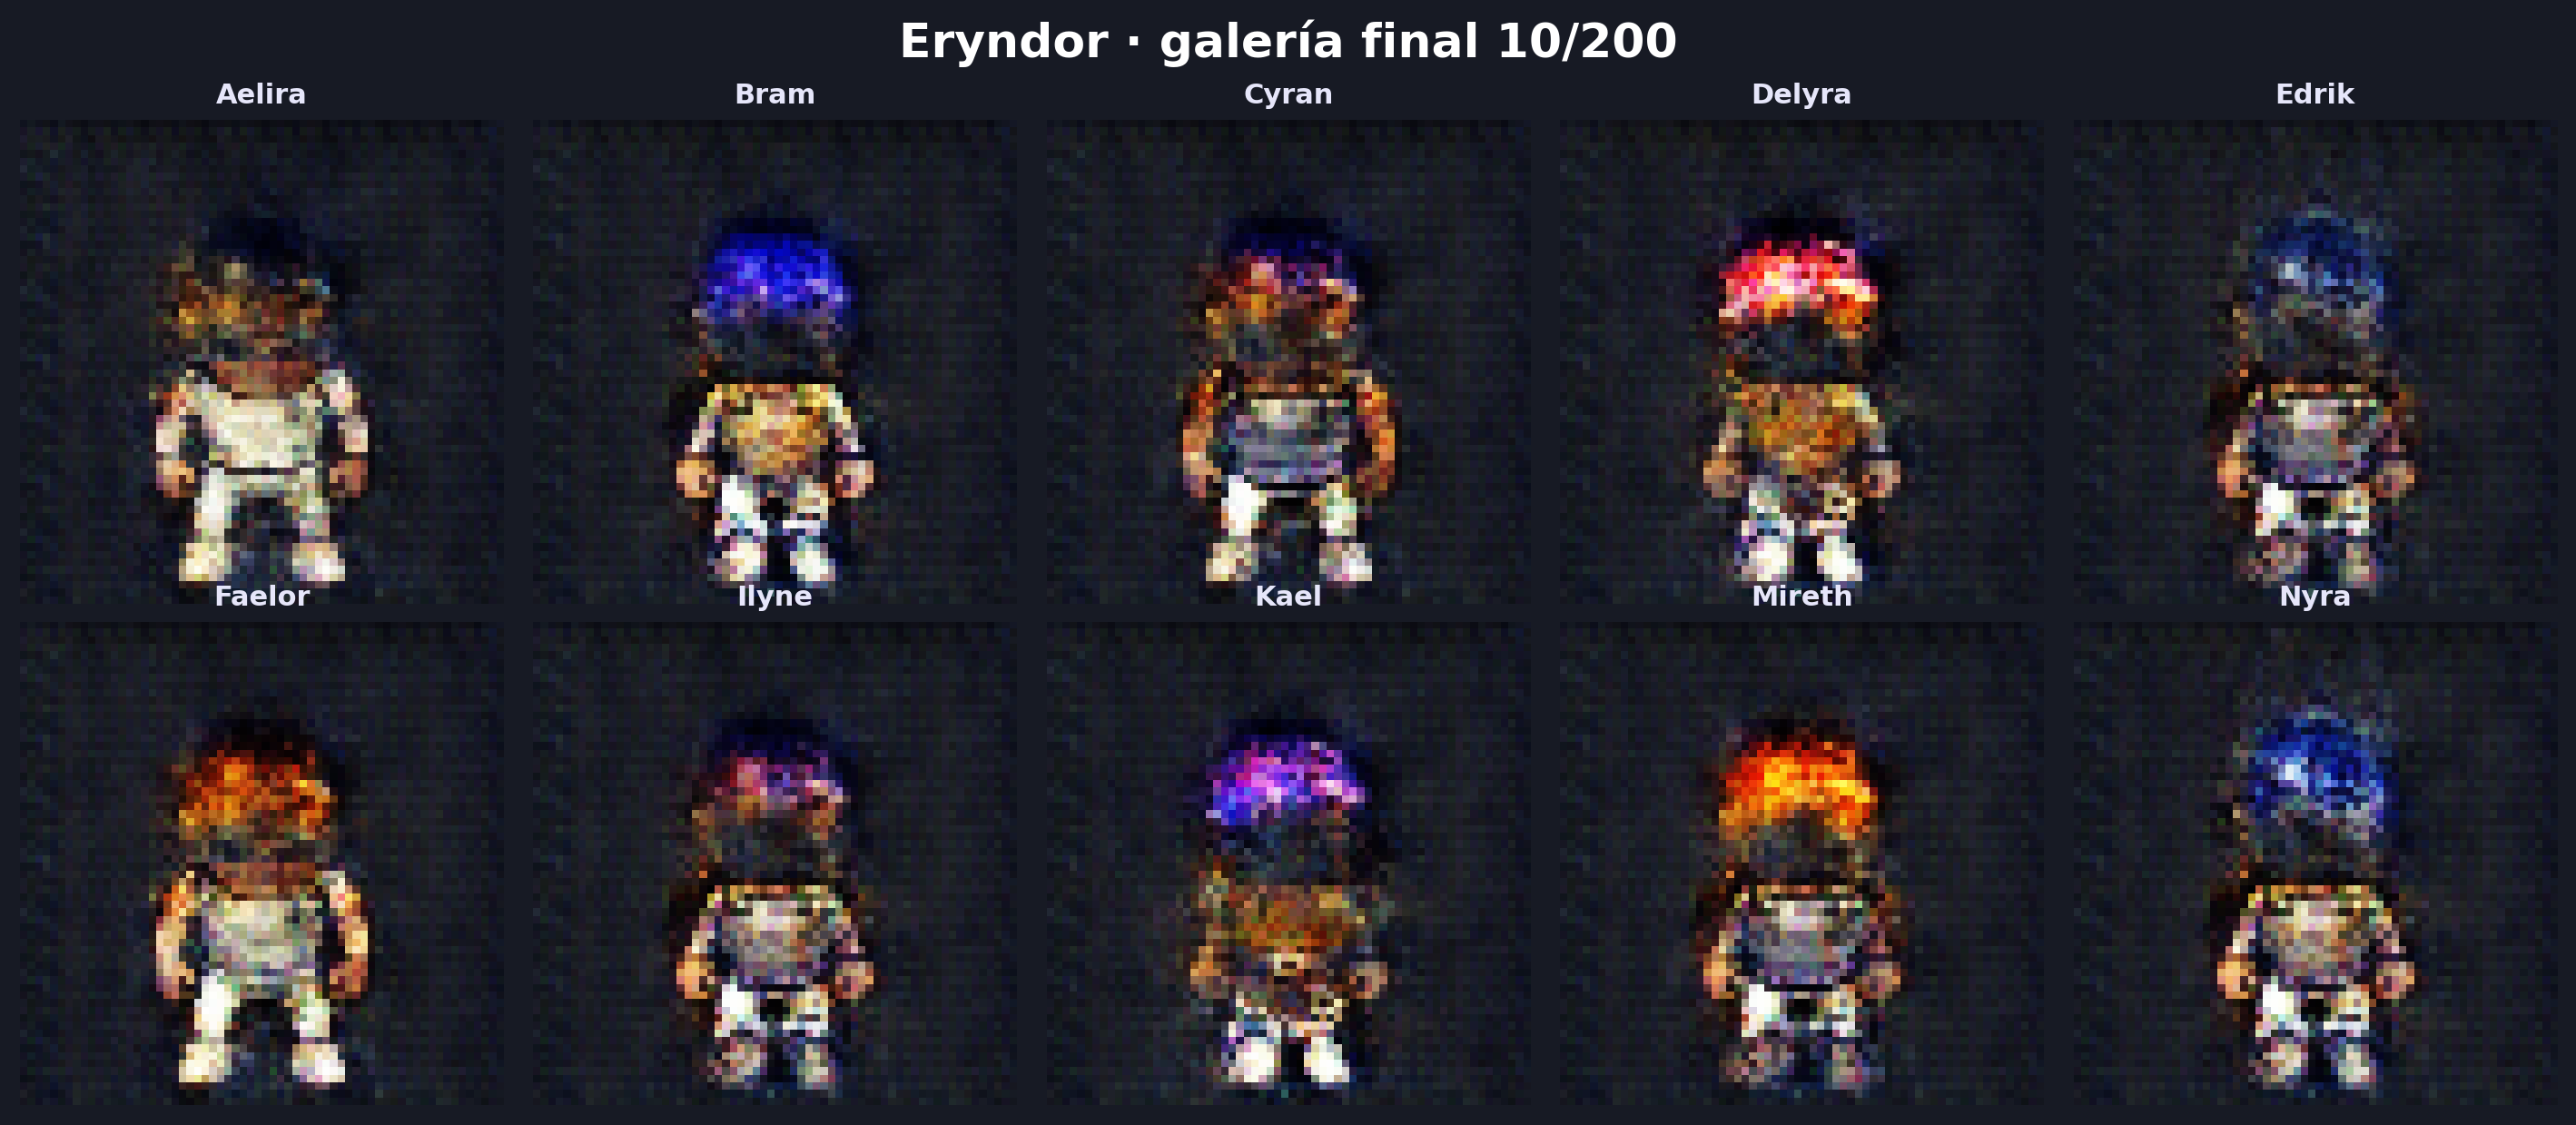
\includegraphics[width=8.95in,height=4.75in,keepaspectratio]{../artifacts/gallery/final_gallery_grid.png}
  \end{minipage}\hfill
  \begin{minipage}[t]{2.7in}
    \eyebrow{Procedencia}\par\vspace{0.12in}
    Modelo: \textbf{\FinalExperiment}\\[8pt]
    Selección: \textbf{\SelectionRate}\\[8pt]
    Delta al regenerar: \textbf{\RegenerationDelta}\\[15pt]
    Cada PNG conserva su vector $z$, índice, semilla, SHA-256, vecino y métricas.
  \end{minipage}
\else
  \vspace{0.75in}
  \statuspending{Se requieren checkpoints de 60 épocas y un modelo seleccionado. Estado actual: A=\BaselineEpoch, B=\HingeEpoch, C=\SpectralEpoch.}
\fi
}

% 10
\slide{09 · Evidencia 3: prueba de vecinos más cercanos}{
\ifgalleryready
  \begin{minipage}[t]{9.0in}
    \vspace{0pt}
    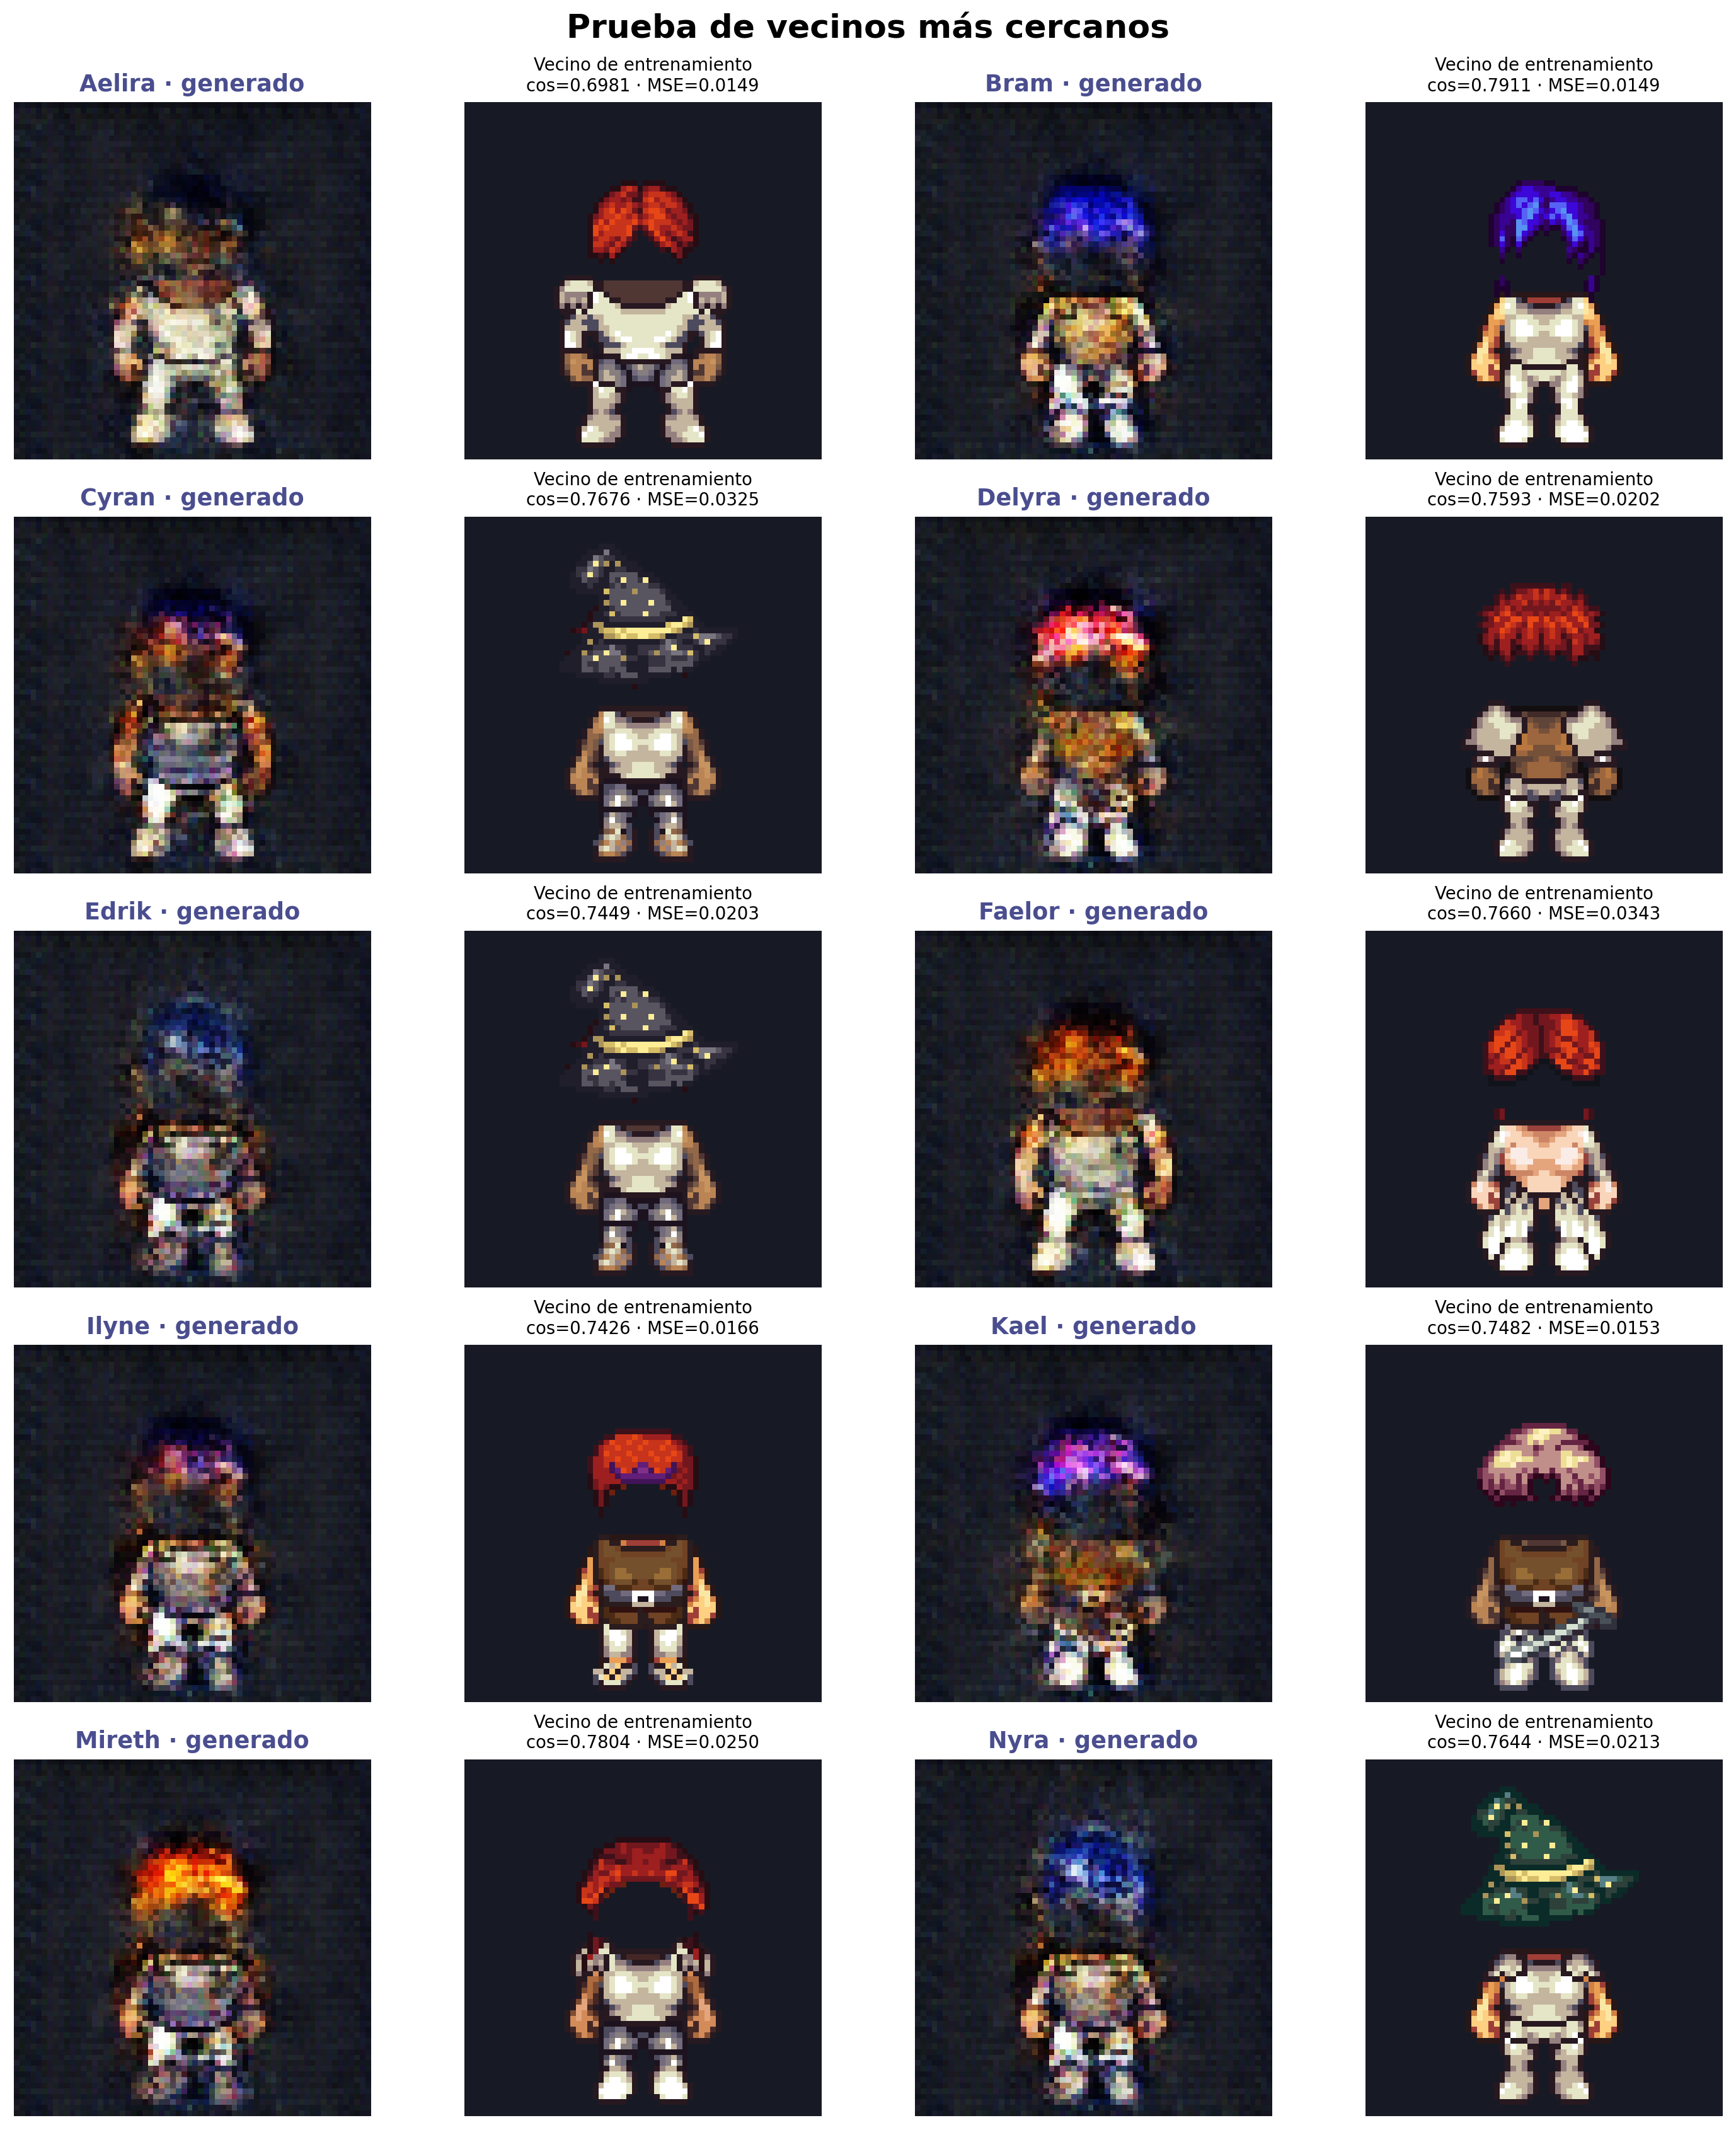
\includegraphics[width=8.9in,height=4.75in,keepaspectratio]{../artifacts/gallery/nearest_neighbors.png}
  \end{minipage}\hfill
  \begin{minipage}[t]{2.8in}
    \eyebrow{Lectura}\par\vspace{0.1in}
    ResNet18 sin capa final + similitud coseno; MSE en píxeles como control secundario.\\[12pt]
    Similitud media: \textbf{\MeanNeighborSimilarity}\\[8pt]
    Caso más difícil: \textbf{\HardestCharacter}\\[4pt]
    coseno: \textbf{\HardestSimilarity}\\[14pt]
    Un personaje casi idéntico a su vecino no se defiende como nuevo.
  \end{minipage}
\else
  \vspace{0.6in}
  \statuspending{El código de ResNet18, similitud coseno, MSE y figura lado a lado está probado; faltan diez imágenes GAN válidas.}\par
  \vspace{0.22in}
  {\small\color{Lavender}\textbf{Tasa declarada prevista:} 10 elegidos de 200 generados = 5\%.}
\fi
}

% 11
\slide{10 · Conclusiones, limitaciones y reflexión}{
\begin{minipage}[t]{5.68in}
  \eyebrow{Lo que sí sabemos}\par\vspace{0.1in}
  \colorbox{CosmicBlue}{\parbox[c][3.8in][c]{5.68in}{\hspace{0.25in}\parbox{5.12in}{
    \textbf{•} Dataset reproducible, sin duplicados y totalmente acreditado.\\[9pt]
    \textbf{•} DCGAN, BCE, hinge y spectral norm funcionan con gradientes finitos.\\[9pt]
    \textbf{•} Checkpoints y semillas restauran exactamente el estado.\\[9pt]
    \textbf{•} La fase 5 impide publicar resultados incompletos.\\[9pt]
    \ifgalleryready
      \textbf{•} La galería validada se regenera con delta RGB \RegenerationDelta.
    \else
      \textbf{•} Todavía no hay evidencia para afirmar que la GAN aprendió personajes.
    \fi
  }}}
\end{minipage}\hfill
\begin{minipage}[t]{5.68in}
  \eyebrow{Limitaciones y reflexión final}\par\vspace{0.1in}
  \colorbox{Obsidian}{\parbox[c][3.8in][c]{5.68in}{\hspace{0.25in}\parbox{5.12in}{
    Una sola pose, bases anatómicas compartidas y embeddings ImageNet aplicados a pixel art limitan la generalización.\\[13pt]
    \ifgalleryready
      \textbf{\HardestCharacter} fue el caso más difícil de defender como nuevo (cos=\HardestSimilarity). Ese vecino muestra qué rasgos del universo aprendió la GAN y cuáles pudo recombinar demasiado literalmente.
    \else
      \textbf{Reflexión pendiente:} solo podrá responderse después de identificar el personaje con mayor similitud frente a su vecino real.
    \fi
  }}}
\end{minipage}
}

% 12
\slide{11 · Matriz de evidencias}{
\scriptsize
\renewcommand{\arraystretch}{1.32}
\begin{tabularx}{11.95in}{>{\bfseries\color{MineralCyan}}p{1.75in} p{0.58in} X X}
  Evidencia & Diap. & Conclusión & Limitación\\[3pt]
  \hline
  Universo y datos & 2--3 & Mundo y dataset coherentes, abiertos y auditados. & Una pose y bases anatómicas compartidas.\\
  Arquitectura GAN & 4 & Contratos tensoriales, pérdidas y checkpoints validados. & Calidad visual pendiente de entrenamiento completo.\\
  Pérdida y estabilidad & 5--8 & Comparación A/B/C cambia una sola variable. & Estado actual 1/60; no existe ganador.\\
  Ruido fijo & 6 & Las tres variantes siguen en textura temprana. & Faltan hitos 5, 10, 20, 40 y 60.\\
  Curvas interpretadas & 7--8 & D domina al inicio; no se confunde $L_D\approx0$ con éxito. & Una época no describe la dinámica final.\\
  Galería + 10/200 & 9 & \ifgalleryready Galería validada y tasa declarada.\else Pipeline listo y bloqueo correcto.\fi & \ifgalleryready Selección humana inevitable.\else No hay PNG finales todavía.\fi\\
  Vecinos cercanos & 10 & \ifgalleryready Novedad medida con coseno y MSE.\else Código implementado sin resultados fabricados.\fi & ResNet18 no fue entrenada específicamente para pixel art.\\
  Conclusión/reflexión & 11 & Alcance y fallos declarados con honestidad. & La respuesta final depende de la galería validada.\\
\end{tabularx}
\vspace{0.2in}
{\scriptsize\color{Lavender}
Fuentes: Goodfellow et al. (2014), Generative Adversarial Nets; Universal LPC Spritesheet Character Generator; LPC Style Guide.\par
Asistencia de IA declarada en README.md. Ninguna imagen de la galería procede de un generador externo.
}
}

\end{document}
